%!TEX root = ../dissertation.tex

\chapter{Results Discussion}

\newthought{Lorem ipsum dolor sit amet}, 

\section{Natural Course} 
In order to test the models used for the g-formula method, a natural course study was performed.  This involved simulating the data directly using the models being used in the g-formula method.  Additionally, a model for the treatment variable had to be created as well, giving the following three models, 
\begin{align} 
Logit \big[Y \mid \overline{A}_t, \overline{L}_t \big] &= \theta_{0} + \theta_1 A_{t} + \cdots + \theta_j A_0 + \theta_{j+1} L_t + \cdots + \theta_{j+k} L_0  \\ 
logit[L_k \mid \overline{L}_{k-1}, \overline{A}_{k-1}] &= \gamma_0 + \gamma_1 L_{k-1} + \gamma_2 L_{k-2} + \gamma_3 L_{k-3}  + \gamma_4 A_{k-1} + \gamma_5 A_{k-2} + \gamma_6 A_{k-3} \\ 
logit[A_k \mid \overline{L}_{k}, \overline{A}_{k-1}] &= \delta_0 + \delta_1 L_{k} + \delta_2 L_{k-1} + \delta_3 A_{k-1} + \delta_4 A_{k-2} 
\end{align} 

Five new data populations were simulated to determine the natural course of these models.  Table \ref{naturalcourse} below compares the true mean of the original data frame and the average across the five simulated dataframes.  


\begin{table}[h!]
\centering
\begin{tabular}{c | c c c}
Variable & True Mean & \shortstack{Natural Course\\ Average Mean} & \shortstack{Natural Course \\95\% CI} \\ 
\hline \\
$\mathbb{E}[Y]$ & 0.714 & 0.719 & (0.705, 0.733) \\ \\
$\mathbb{E}[A]$ & 0.848 & 0.847 & (0.840, 0.854) \\ \\
$\mathbb{E}[L]$ & 0.833 & 0.811 & (0.793, 0.830) 
\end{tabular} \\
\centering
\caption{Hi? \label{naturalcourse}}
\end{table}

The results of the natural course show that the models chosen appear to estimate the data quite well.  Not only are the means close to the true mean, but the variance is low enough that our confidence intervals all cover the true mean.  Therefore, it can be concluded that these models are a good choice for use in the g-formula.  

\section{Simulation of the Two Methods} 
As discussed in Section \ref{VarianceBootStrap}, a simulation of 1,000 iterations was performed.  Each iteration of this simulation consisted of creating a new dataset and obtaining both the g-formula estimate and the doubly robust estimate for the causal treatment effect.  The results of these simulations can be seen below in Table \ref{simdata} 

\begin{table}[h!]
\centering
\begin{tabular}{c | c c c }
Method & \shortstack{Average Causal \\ Treatment Effect} & \shortstack{Variance\\ of Estimate} & \shortstack{95\% Conf. Int.\\ of Estimate} \\ 
\hline \\
G-Formula & 0.0033 & 0.00024&(-0.00063,0.00128)\\ \\ 
Doubly Robust & 0.00026 &0.00079 & (-0.00149, 0.00212)
\end{tabular} \\
\centering
\caption{Hi? \label{simdata}}
\end{table}

\begin{figure}
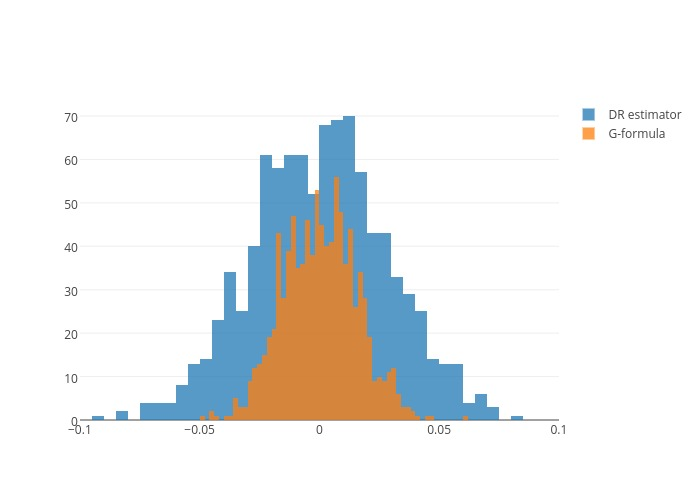
\includegraphics[width = \linewidth]{figures/overlaid_histogram.jpeg}
\caption{}
\label{bighistogram}
\end{figure} 




\section{Confirming Double Robustness} 
Ten simulations were performed in order to test the double robustness of the ``doubly'' robust estimator.  Four different setups were tested: 
\begin{itemize} 
\item Using the correct model for both user specified functions, $\hat{\mathbf{\alpha}}$ and $s_{m-1}$ 
\item Using an intentionally misspecified model for $\hat{\mathbf{\alpha}}$ while keeping the correct model for $s_{m-1}$ 
\item Using an intentionally misspecified model for $s_{m-1}$ while keeping the correct model for $\hat{\mathbf{\alpha}}$
\item Using intentionally misspecified models for both $\hat{\mathbf{\alpha}}$ and $s_{m-1}$ 
\end{itemize} 

The misspecified models used were as follows, 
\begin{align} 
f(A_m \mid \overline{L}_m, \overline{A}_{m-1}; \hat{\mathbf{\alpha}}) &= \alpha'_{0} + \alpha'_{1} \cdot L_{m-3} + \alpha'_{2} \cdot A_{m-3} \\ 
s_{m}(\overline{L}_{m}, \overline{A}_{m};\mathbf{\beta}_{m}) &= \theta'_0 + \theta'_1 A_{m} +\theta'_2 A_{m-4} + \theta'_3 L_{m-4} 
 \end{align} 

\begin{table}[h!]
\centering
\begin{tabular} {c | c  c c}
Models & Mean & Variance & CI \\ 
\hline  \\
Both models correctly specified & 0.0061 & 0.001& (-0.007, 0.019)\\ \\
$\hat{\mathbf{\alpha}}$ correct, $s_{m-1}$ misspecified & 0.011 & 0.001& (-0.003, 0.025)\\ \\
$\hat{\mathbf{\alpha}}$ misspecified, $s_{m-1}$ correct & 0.012 & 0.001& (-0.002, 0.026) \\ \\
Both models misspecified & 0.048 & 0.047 & (-0.037, 0.133) 
\end{tabular} \\
\centering
\caption{Hi?}
\end{table}

\begin{figure}
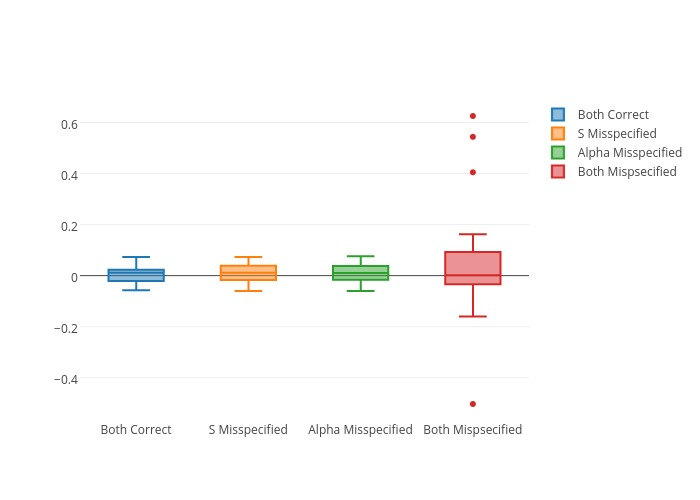
\includegraphics[width = \linewidth]{figures/boxplot.jpg}
\caption{}
\label{boxplot}
\end{figure} 




\section{Testing Multiple Robustness} 

\begin{table}[h!]
\centering
\begin{tabular} {c | c  c c}
Model Correctly Specified & \shortstack{Average Causal \\ Treatment Effect}  & Variance & \shortstack{95\% Conf. Int.\\ of Estimate} \\ 
\hline  \\
$\pi_3, \dots, \pi_K$ & -0.0025 & 0.0013 & (-0.009, 0.005)  \\ 
$\pi_3, \dots, \pi_{K-1}, s_K$ & -0.0054 & 0.0010& (-0.012, 0.001)\\ 
$\pi_3, \dots, \pi_{K-2}, s_{K-1}, s_K$ & -0.0046 & 0.0010&(-0.011, 0.002)\\ 
$\pi_3, \dots, \pi_{K-3}, s_{K-2} , s_{K-1}, s_K$ & -0.0045 &0.0009 & (-0.010, 0.001)\\ 
$\pi_3, \dots, \pi_{K-4}, s_{K-3}, \dots s_K $ & -0.0044 &0.0009& (-0.010, 0.002) \\ 
$\pi_3, \dots, \pi_{K-5}, s_{K-4}, \dots s_K $ & -0.039 &0.0009& (-0.010, 0.002)\\ 
$\pi_3, \dots, \pi_{K-6}, s_{K-5}, \dots s_K $ & -0.0029 & 0.0009&(-0.009, 0.003) \\ 
$\pi_3, \dots, \pi_{K-7}, s_{K-6}, \dots s_K $ & -0.0006 & 0.0010& (-0.007, 0.006)\\ 
$\pi_3, s_{4}, \dots s_K $ & 0.0025 & 0.0011 & (-0.004, 0.009) \\ 
$s_3, \pi_4, \dots \pi_K$ & 0.0033 & 0.0881 & (-0.055, 0.061)\\ 
$s_3, s_4, \pi_5, \dots \pi_K$ & 0.0262 & 0.0214  & (-0.002, 0.055)\\ 
$s_3, s_4, s_5, \pi_6, \dots \pi_K$ & 0.0035 & 0.0100 & (-0.016,0.023) \\ 
$s_3, \dots s_6, \pi_7, \dots \pi_K$ & 0.0209 &0.0206 & (-0.007, 0.049)\\ 
$s_3, \dots s_7, \pi_8, \dots \pi_K$ & 0.0129 &  0.0195   & (-0.014, 0.040) \\ 
$s_3, \dots s_8, \pi_9, \dots \pi_K$ & -0.0145 &0.0129   & (-0.037, 0.008) \\ 
$s_3, \dots s_9, \pi_{10}, \pi_K$ & -0.0020 & 0.0015 & (-0.009, 0.006)\\ 
$s_3, \dots s_{10}, \pi_K$ & -0.0018& 0.0013 & (-0.009,  0.005)\\
$s_3, \dots s_K$ & -0.0024 & 0.0013& (-0.009, 0.005)\\ 
\end{tabular} \\
\centering
\caption{Hi?}
\end{table}

\begin{figure}
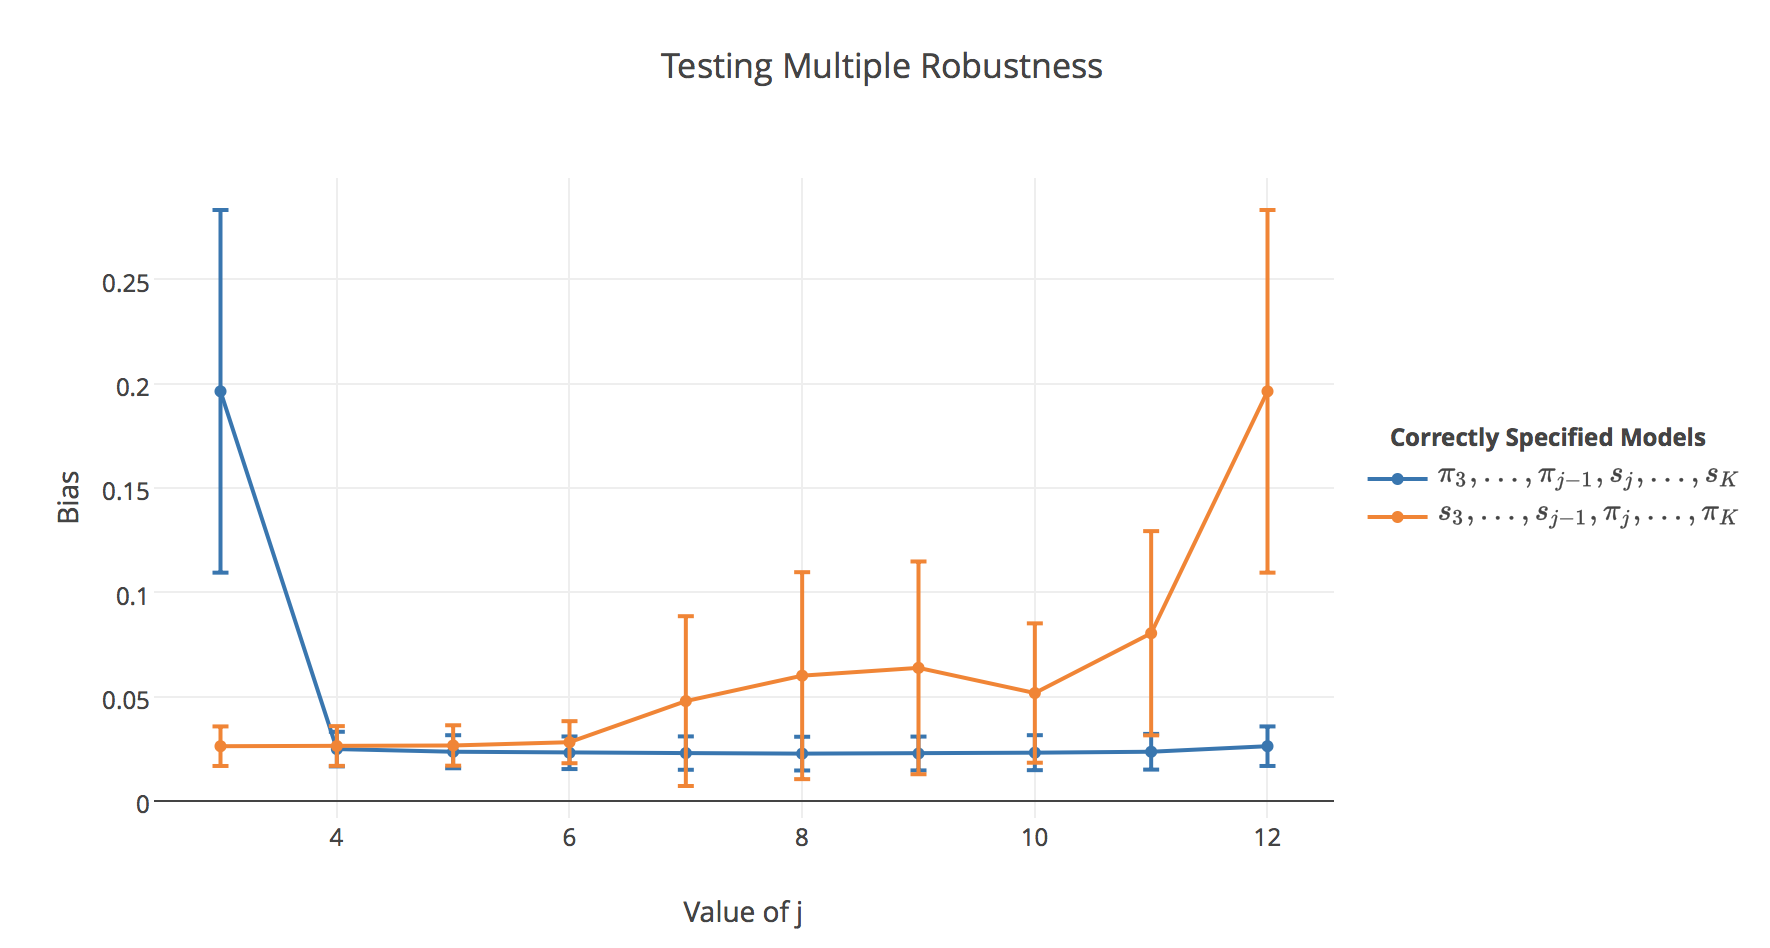
\includegraphics[width = \linewidth]{figures/multiplerobust.png}
\caption{}
\label{multirobust}
\end{figure} 

